\section{Realisierung}
\label{sec:Realisierung}

Wie im Anhang (\secref{sec:Entscheidung-Programmiersprache}) beschrieben und begründet, wird \texttt{px} mit \textsc{Go} umgesetzt. Da die Standard Library von \textsc{Go} sehr umfassend ist, die mit dem Package \texttt{net/http} über einen mächtigen HTTP-Client (und Server) verfügt, wird nur eine Fremdkomponente (Zugriff auf den Keystore) eingesetzt.

Enorm hilfreich in der Umsetzung war Standardwerk zu \textsc{Go} \cite{gopl}, das nicht nur die Programmiersprache beschreibt, sondern auch deren idiomatischen Gebrauch.

\subsection{Architektur: Package-Übersicht}

\textsc{Go}-Code wird in sogenannte Packages aufgeteilt. Da das Projekt in \textsc{GitLab} \texttt{px} heisst, wird das Hauptpackage als \texttt{px} benannt. Im Root-Verzeichnis befindet sich kein \textsc{Go}-Code.\footnote{\texttt{px.go} beinhaltet bloss eine Package-Deklaration mit einem entsprechenden Kommentar.} Dieser ist in verschiedenen Unterverzeichnissen (\texttt{requests}, \texttt{tokenstore}, usw.) abgelegt. Die Dateien in den Unterpackages deklarieren ihre Packagezugehörigkeit jeweils mit dem unmittelbaren Überverzeichnis, also beispielsweise nicht \texttt{px/tokenstore}, sondern nur \texttt{tokenstore}. Bei der Verwendung der Packages hingegen wird der ganze Pfad angegeben: \texttt{px/tokenstore}.

Der Code für das ausführbare Programm (\texttt{px.go}) befindet sich gemäss Konvention\footnote{\url{https://github.com/golang-standards/project-layout\#cmd}} im \texttt{cmd}-Unterverzeichnis \cite[S. 12]{powerful-cli-apps-in-go}. Das Package heisst jedoch nicht \texttt{cmd}, sondern \texttt{main}, und verfügt über eine Funktion namens \texttt{main} als Haupteinstiegspunkt. Somit ist \texttt{px} als Library, und \texttt{cmd/px.go} als Client dieser Library zu verstehen.\footnote{Da sich nur knapp ein Viertel des Programmcodes im Client-Teil befinden, könnte auf Basis der \texttt{px}-Library recht einfach ein alternativer Client umgesetzt werden.} Die Projektstruktur ist auf der linken Seite der \imgref{img:Komponentendiagramm} zu sehen. Die einzelnen Packages haben folgende Verantwortlichkeiten:

\begin{figure}
    \centering
    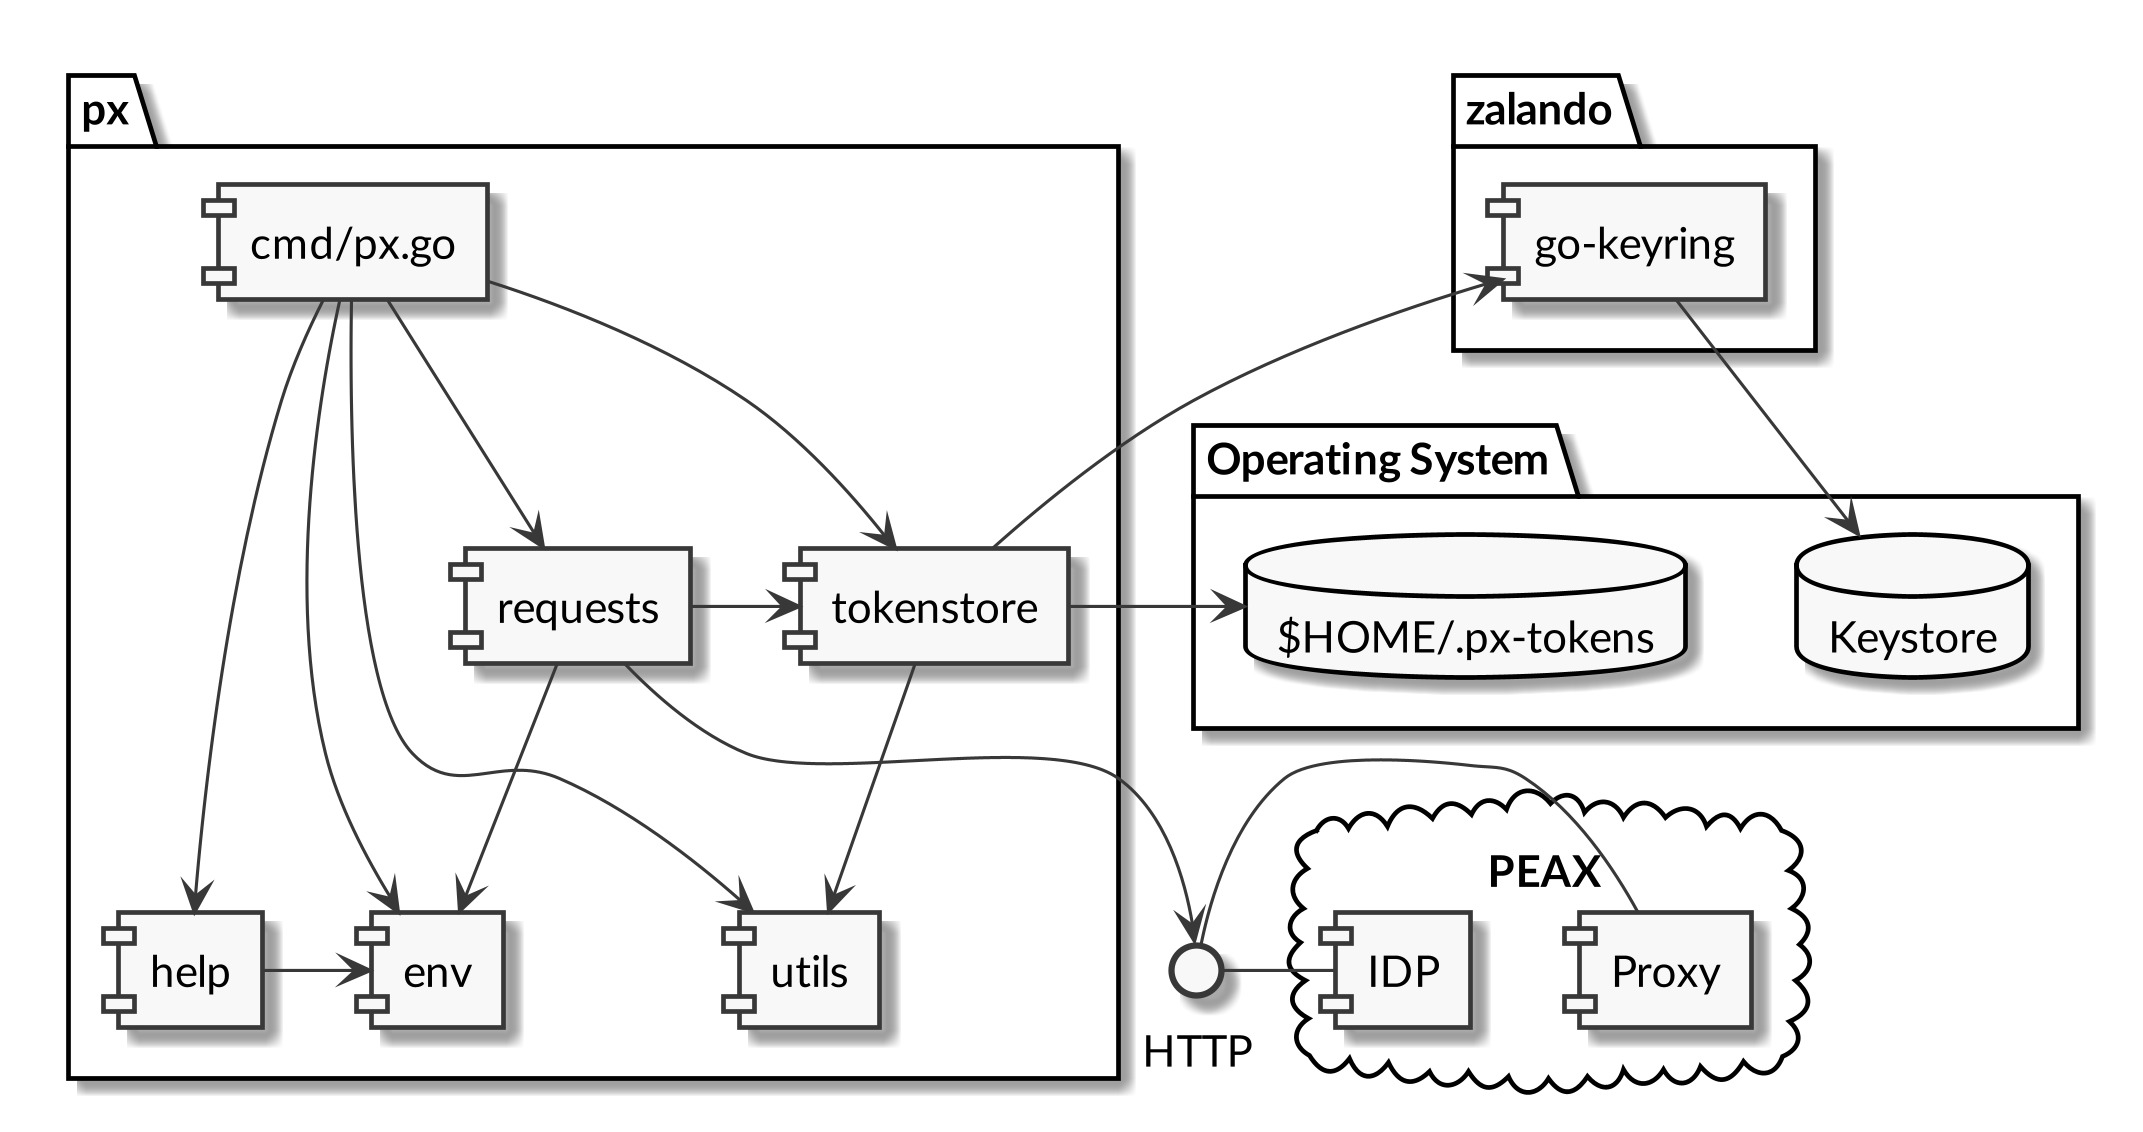
\includegraphics[width=\linewidth]{pics/komponentendiagramm.png}
    \caption{Die Package-Struktur von \texttt{px} (Komponentendiagramm)}
    \label{img:Komponentendiagramm}
\end{figure}

\begin{description}
    \item[\texttt{env}] Die Umgebungen (\secref{sec:Umgebungen}) sind in diesem Package aufgelistet. Jede Umgebung verfügt über ein URL-Schema, womit (via Proxy) auf das Backend und direkt auf den IDP zugegriffen werden kann. Verschiedene Funktionen bieten die Möglichkeit, URLs für den Ressourcenzugriff anhand der jeweiligen Umgebung und weiterer Parameter zu erzeugen, was mit dem Unit Test \texttt{env\_test.go} überprüft wird. Die Standardeinstellung, welcher Keystore (sicher/unsicher) zu verwenden ist, wird statisch pro Umgebung definiert.
    \item[\texttt{help}] Dieses Package umfasst die Hilfetexte. Zu jedem Befehl gibt es jeweils eine kurze, einzeilige Beschreibung, und einen ausführlichen Hilfetext. Dieses Package importiert das \texttt{env}-Package, damit bei der Hilfe zum Login-Befehl (\texttt{px login}) die verfügbaren Umgebungen automatisch aufgelistet werden können.
    \item[\texttt{tokenstore}] Hier sind zentrale Datenstrukturen für das Token-Handling mit dazugehörigen Funktionen definiert. Die Datenstruktur \texttt{TokenPair} dient zur lokalen, persistenten Speicherung von Tokens. Sie wird auf Basis einer \texttt{TokenResponse} aufgebaut, indem Informationen extrahiert und anhand von Kontextinformationen ergänzt. Die Datenstruktur \texttt{TokenStore} speichert pro Umgebung und Token-Typ (\texttt{agent}, \texttt{user}) ein \texttt{TokenPair} ab. Der \texttt{TokenStore} wird als JSON-Struktur serialisiert und im \texttt{\$HOME}-Verzeichnis des Benutzers abgespeichert. Der Zugriff auf den sicheren Keystore ist ebenfalls hier implementiert.
    \item[\texttt{requests}] In diesem Package sind die eigentlichen Zugriffe auf die API via HTTP umgesetzt. Hier sind Datenstrukturen für die Credential-Payloads mit dazugehörigen Funktionen definiert, die für Login-Vorgänge verwendet werden (\texttt{credentials.go}. Für die verschiedenen Befehle (\texttt{login}, \texttt{get}, \texttt{upload} usw.) sind hier dazugehörige Funktionen definiert. Der transparente Retry-Mechanismus ist ebenfalls hier implementiert (\texttt{requests.go}). Das Package \texttt{tokenstore} wird verwendet, um die Requests mit den notwendigen Authentifizierungsinformationen (\texttt{Authentication}-Header) auszustatten.
    \item[\texttt{utils}] Dieses Package umfasst verschiedene Funktionen, die von verschiedenen anderen Packages und vom Hauptprogramm verwendet werden, jedoch nicht direkt zu den jeweiligen anderen Packages gehören. Die Eingabeaufforderung für Passwörter (sicher über ein SSH-Terminal, d.h. ohne Echo) ist etwa hier umgesetzt (\texttt{pwinput.go} und \texttt{pwinput\_windows.go}\footnote{Aufgrund eines offenen Fehlers (\url{https://github.com/golang/go/issues/34461}) funktioniert die sichere Passworteingabe nicht unter \textsc{Windows}. Aus diesem Grund wird mithilfe eines Build Constraints (\url{https://golang.org/pkg/go/build/\#hdr-Build\_Constraints}) für den \textsc{Windows}-Build eine unsichere Variante, für alle anderen Betriebssysteme die sichere Variante verwendet.}). Weiter gibt es Funktionen zum automatischen Ermitteln des MIME-Types einer Datei, und eine Funktion zur rekursiven Auflisten lesbarer Dateien in einem Unterverzeichnis.
    \item[\texttt{cmd/px.go}] Dies ist der eigentliche Command Line Client mit der Einstiegsfunktion \texttt{main}. Die zur Verfügung stehenden Befehle weden in einer Map namens \texttt{commands} abgespeichert, wobei der Befehlsname den Key bildet, und der Wert eine Datenstruktur bestehend aus einer Funktionsreferenz, dem einzeiligen Infotext und dem längeren Hilfetext (siehe Package \texttt{help}) zusammengesetzt ist. Die \texttt{main}-funktion prüft, ob der eingegebene Befehl in der Map gefunden wurde, und führt diese dann aus. Jede dieser Command-Funktionen nimmt den \texttt{TokenStore} als Argument entgegen, und gibt einen optionalen Fehler zurück.\footnote{Die Befehle \texttt{help} und \texttt{env} bilden eine Ausnahme.} Der \texttt{TokenStore} wird zu Beginn von \texttt{main} aus \texttt{\$HOME/.px-tokens} geladen, und am Ende (mit möglichen Änderungen) wieder in diese Datei zurückgeschrieben.\footnote{Die sicher verwahrten Tokens werden bei Bedarf, d.h. bei einem entsprechenden Request, nachgeladen.} Die einzelnen Command-Funktionen sind selber für ihre Seiteneffekte (Ausgabe möglicher Payloads) verantwortlich. Die Fehlerausgabe wird über die Rückgabe eines Fehlers in \texttt{main} abgehandelt. Die Flags sind ebenfalls für jeden Befehl eigens definiert, wobei Gemeinsamkeiten in Hilfsfunktionen und Konstanten (Beschreibungstexte) ausgelagert sind. Das Parsen der Kommandozeilenargumente wird vom sehr mächtigen und komfortablen \texttt{flag}-Package übernommen, das Teil der Standard Library von \textsc{Go} ist. Tritt bei der Programmausführung ein Fehler auf, wird einerseits eine Fehlermeldung auf \texttt{stderr} geschrieben, andererseits der Rückgabewert \texttt{1} an den aufrufenden Prozess zurückgegeben.\footnote{Im Gegensatz zu \texttt{0}, das für eine erfolgreiche Ausführung steht.} Dieser Rückgabecode wird in den Testskripts über die Shell-Variable \texttt{\$?} geprüft.
\end{description}

\subsection{Zwei-Faktor-Authentifizierung}

\begin{figure}
    \centering
    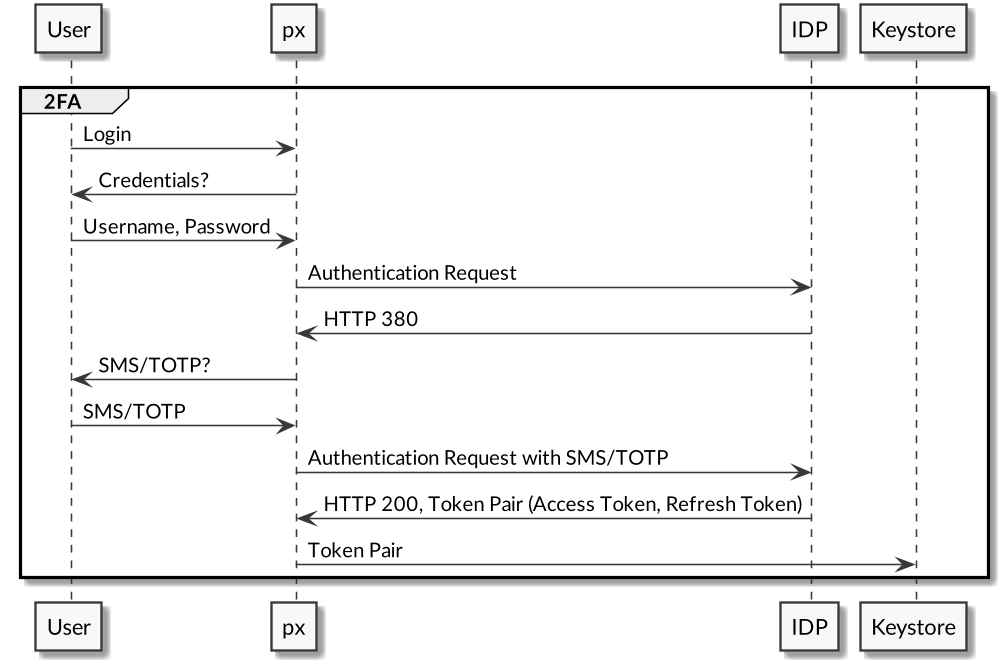
\includegraphics[width=\linewidth]{pics/sequence-2fa.png}
    \caption{Sequenzdiagramm: Der Ablauf der Zwei-Faktor-Authentifizierung mit SMS oder OTP}
\end{figure}

\subsection{Token Store}
\label{sec:Realisierung-Token-Store}

TODO: sicher und unsicher, Datenstruktur

\subsubsection{Fremdkomponente \texttt{zalando/go-keyring}}

\subsection{Retry-Mechanismus}
\label{sec:Retry-Mechanismus}

\begin{figure}
    \centering
    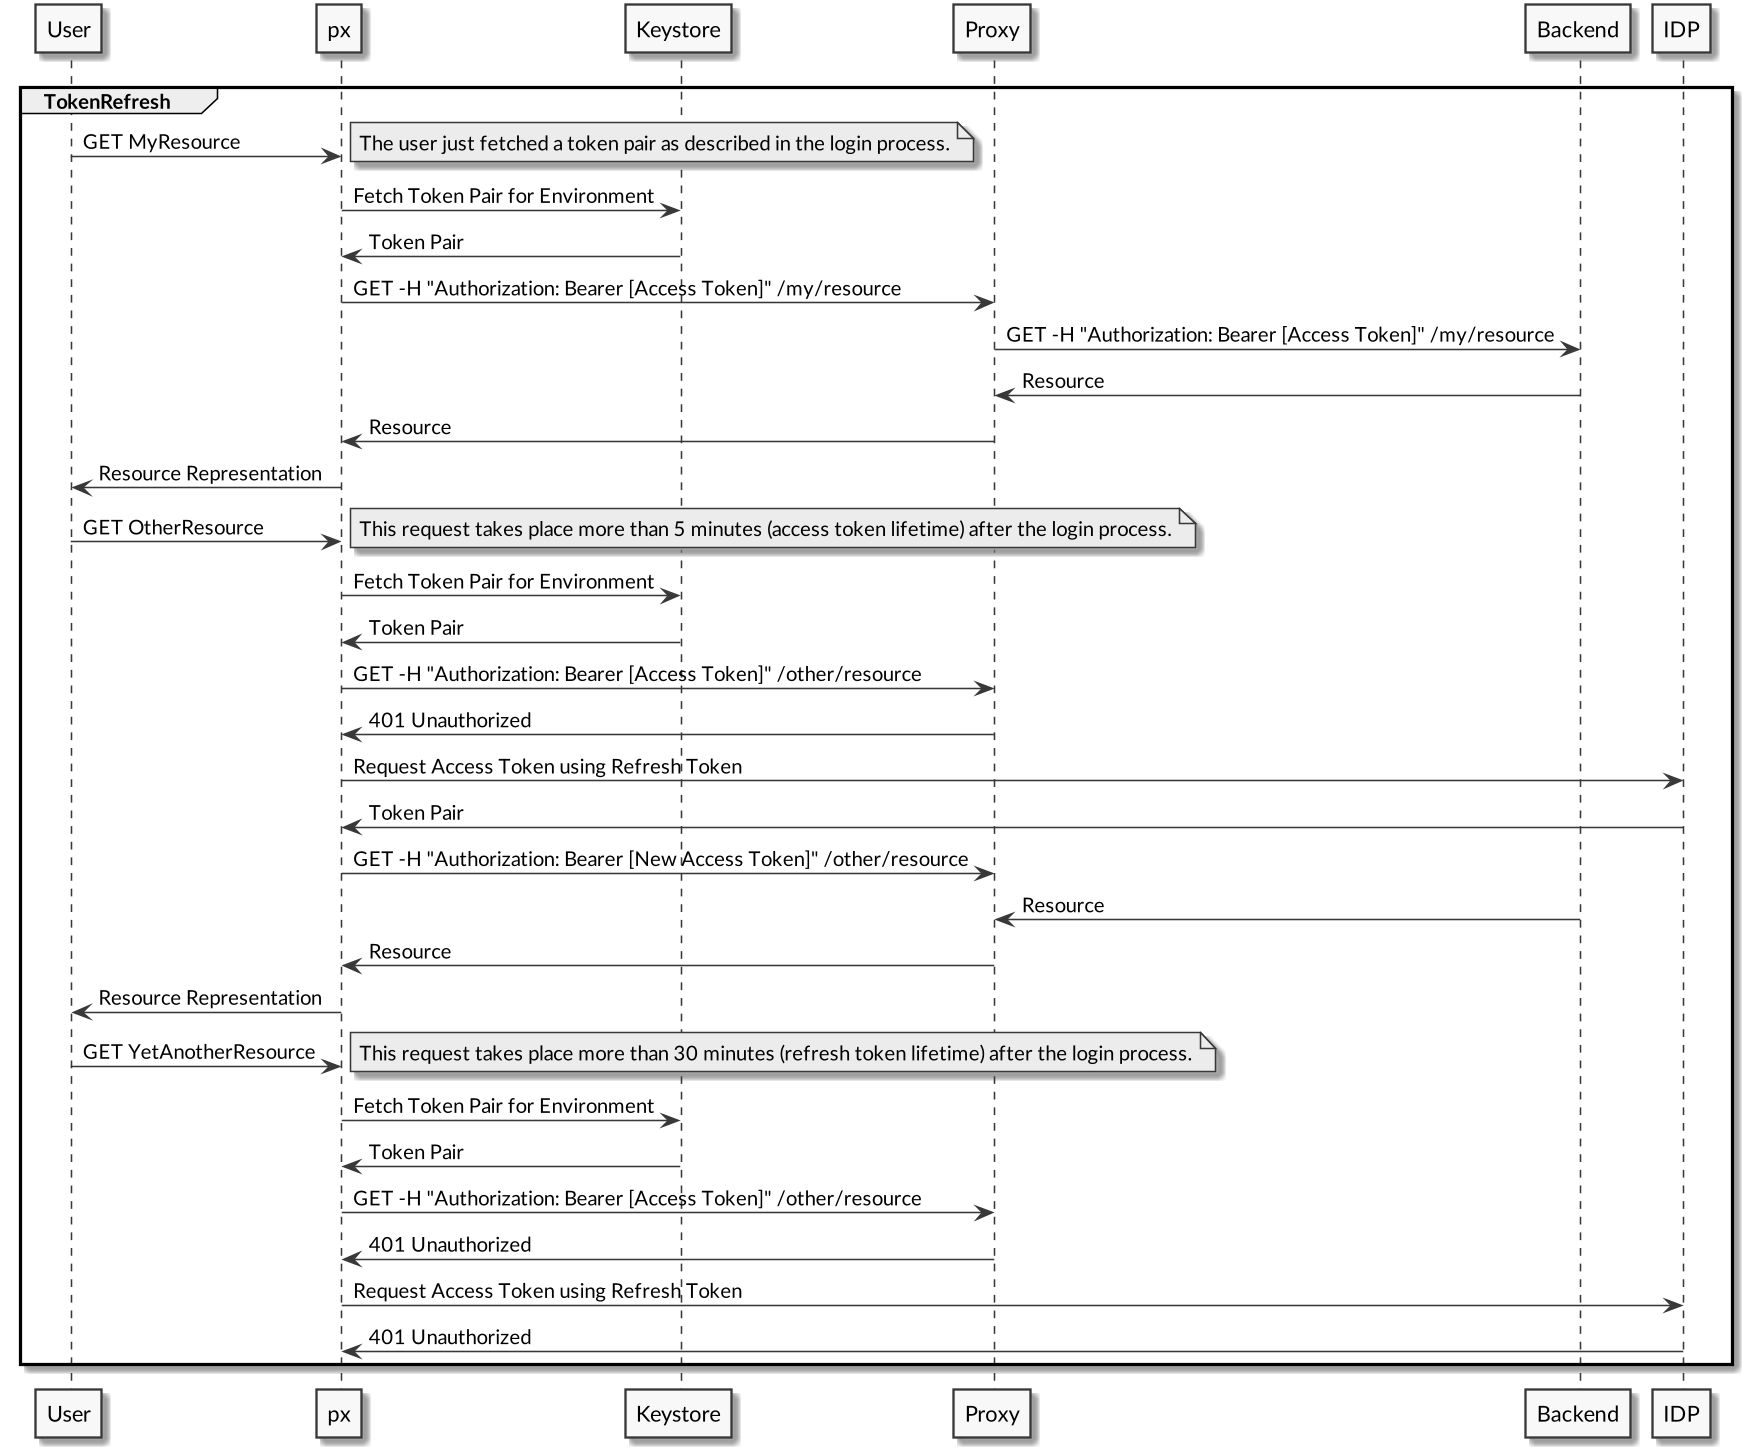
\includegraphics[width=\linewidth]{pics/sequence-retry.png}
    \caption{Sequenzdiagramm: Der für den Benutzer transparente Retry-Mechanismus mit einem Token Pair, das im Hintergrund automatisch aktualisiert wird}
\end{figure}
